% ============================================================
%  MRL 2026 camera-ready. Accepted 2026-09-21, submission #93.
%  [final] is the camera-ready option: de-anonymised, no line numbers.
%  [review] rebuilds the anonymised submission; note that Code and Data
%  Availability names the repo URL, which [review] does not mask.
% ============================================================

\documentclass[11pt]{article}

\usepackage[final]{acl}

\usepackage[T1]{fontenc}
\usepackage[utf8]{inputenc}
\usepackage{times}
\usepackage{latexsym}
\usepackage{microtype}
\usepackage{booktabs}
\usepackage{graphicx}
\usepackage{amsmath}
\usepackage{xcolor}
\usepackage{subcaption}
\usepackage{inconsolata}

% ---- Paper metadata ----
\title{A False Positive in Cross-Lingual\\
Unlearning Evaluation}

% Shown in full under [preprint]; masked again if you switch to [review].
\author{
  Mohamed Waseem \\
  Sathyabama Institute of \\ Science and Technology \\
  Chennai, India \\
  \texttt{waseeeem177@gmail.com}
  \And
  Mohammed Fawaz \\
  Sathyabama Institute of \\ Science and Technology \\
  Chennai, India \\
  \texttt{fawaznx97@gmail.com}
}

\begin{document}
\maketitle

% ============================================================
\begin{abstract}
Cross-lingual audits of LLM unlearning ask whether a fact forgotten in one
language remains recoverable in another, and read a small loss increase in
the second language as residual recall.
We show that this inference is unsafe without a control that is routinely
omitted.
Auditing GradDiff unlearning of TOFU fictional-persona facts on
\textsc{Qwen2.5-0.5B} across English, Modern Standard Arabic, Egyptian
Arabic and Hindi, we find the expected signature of leakage: the unlearned
model's forget-set loss rises by $+2.922$ nats in English but only $+0.774$
in MSA, $26\%$ as much.
Measuring the base model as well shows that signature to be an artefact.
English-only fine-tuning left no measurable trace of the facts in the other
three varieties — it raised forget-set loss there, and raised retain-set loss
by an indistinguishable amount — so there is no evidence of cross-lingual
memory for unlearning to have left behind.
Once the never-learned and the uniform-degradation components are removed,
the MSA effect is $+0.054$ nats, $2.5\%$ of English rather than $26\%$.
We argue that a base-model transfer control and a retain-set control are
jointly necessary for any cross-lingual unlearning claim, and report the
audit design that yields them at no additional training cost.
\end{abstract}

% ============================================================
\section{Introduction}
\label{sec:intro}

The \emph{right to be forgotten} \citep{cao2015towards} motivates machine
unlearning: the ability to remove specific training knowledge from a
deployed model without full retraining.
Recent work operationalises this for LLMs through loss-based
forgetting \citep{yao2023llmunlearning,zhang2024npo} evaluated on
held-out forget sets in a single language.

A critical blind spot remains: \textbf{LLMs are trained on multilingual
corpora}, so knowledge stored in one language is partially encoded across
many.
If a method unlearns a fact in English but leaves the same knowledge
retrievable in Arabic, the unlearning is incomplete regardless of what
English-only metrics report.

Prior work has begun to surface this problem.
\citet{choi2024crosslingual} show that knowledge unlearned in one language
can persist in others, and propose an adaptive scheme that assigns
language-dependent weights during unlearning.
\citet{farashah2026multilingual} confirm the phenomenon on Aya-Expanse-8B
\citep{dang2024ayaexpanse} across ten languages spanning five families,
finding that syntactic similarity is the strongest predictor of how much
leakage occurs.

We set out to extend this line to Arabic, which both treat as a single node,
by separating MSA from a dialectal variety. What we report instead is a
problem with how the measurement is made. MSA and Egyptian Arabic do still
separate in our data, but on a quantity that turns out not to be leakage,
and we treat that separation as evidence about the audit rather than about
the varieties.

The standard cross-lingual audit compares an unlearned model against the
fine-tuned model it started from, in each language. A large loss increase in
the unlearning language and a small one elsewhere is read as leakage. That
reading assumes two things which are rarely checked: that the fine-tuned
model knew the fact in the other language to begin with, and that whatever
loss movement does appear there is specific to the forgotten facts rather
than a global side effect of unlearning. Neither assumption survives contact
with a base-model measurement in our setup.

Our audit reproduces the textbook leakage signature — MSA moves $26\%$ as
much as English — and then dissolves it. Fine-tuning on English TOFU did not
teach the model the facts in MSA, Egyptian Arabic or Hindi; it made the model
uniformly worse in all three, on forget and retain facts alike. The residual
MSA movement after unlearning is likewise uniform across forget and retain.
A fact for which no acquisition in Arabic can be demonstrated cannot support a
claim about leakage in Arabic, and an evaluation that omits the base model
cannot tell that situation apart from genuine residual recall.

\paragraph{Contributions.}
\begin{enumerate}
  \item We show that a cross-lingual unlearning audit without a base-model
        transfer control can report substantial leakage where no
        acquisition has been shown, and quantify the gap in our own setup: an
        apparent MSA effect of $26\%$ of English falls to $2.5\%$ once the
        never-learned and uniform-degradation components are removed.
  \item We give the control design that separates them — base
        \emph{and} anchor measurements crossed with forget \emph{and} retain
        probes, in every language — and show it costs no extra training,
        only inference passes over adapters that already exist.
  \item We report the negative transfer result itself: monolingual QLoRA
        fine-tuning of a 0.5B model on 4{,}000 synthetic facts produces no
        measurable cross-lingual acquisition of those facts in three typologically
        varied target languages, which bounds the settings in which
        cross-lingual unlearning can meaningfully be studied at this scale.
\end{enumerate}

% ============================================================
\section{Background and Related Work}
\label{sec:related}

\paragraph{Machine unlearning for LLMs.}
Gradient Ascent (GA) unlearning maximises loss on forget-set examples,
driving the model away from those predictions
\citep{jang2023knowledge}.
GradDiff \citep{liu2022continual}, applied to LLM unlearning by
\citet{yao2023llmunlearning}, augments GA with a retain-set
cross-entropy term to prevent catastrophic forgetting of general capabilities.
Negative Preference Optimisation (NPO) \citep{zhang2024npo} reformulates
the forget objective as preference learning.
All three methods are evaluated exclusively in the unlearning language.

\paragraph{TOFU.}
\citet{maini2024tofu} introduce TOFU (Task of Fictitious Unlearning), a
controlled benchmark of 4,000 question-answer pairs about fictional authors.
Because the facts are synthetic, ground-truth forgetting can be defined
precisely.
The standard evaluation uses forget10 (the 10\% held-out forget split) and
reports loss and ROUGE alongside \emph{forget quality}, a
Kolmogorov--Smirnov test comparing truth-ratio distributions against a
retrained model.

\paragraph{Cross-lingual unlearning.}
\citet{choi2024crosslingual} demonstrate that unlearning in one language does
not erase knowledge in others, and propose an adaptive unlearning scheme with
language-dependent weights.
\citet{doshi2024unlearn} show that unlearned knowledge resurfaces under simple
black-box perturbations of the query, including rephrasing and translating it
into another language.
Most related to our work, \citet{farashah2026multilingual} find that
syntactic distance between languages is the strongest predictor of leakage
magnitude — implying Arabic dialects, which are syntactically closer to MSA
than to English, may leak differently. Their design differs from ours in a
way that matters for the comparison: they fine-tune on every language they
evaluate, so acquisition in each is established by construction, and they
report a retain-only baseline alongside the unlearned model. The gap we
identify does not apply to that setup. It applies to the common case, ours
included, where fine-tuning happens in one language and the audit reports
several.

What these studies share is that the headline comparison is between the
fine-tuned and the unlearned model. The pre-fine-tuning model is used, if at
all, to establish
that the benchmark facts are unknown at the outset; it is not used per
language to establish that fine-tuning made them known in the language the
audit probes. That step is what our results show to be load-bearing. The
closest methodological precedent is \citet{doshi2024unlearn}, who argue that
apparent forgetting is an artefact of the probe and recover the supposedly
unlearned knowledge by perturbing the query. Our claim is the mirror image:
apparent \emph{failure} to forget can equally be an artefact of the probe,
and the same discipline about controls is needed in both directions.

% ============================================================
\section{Experimental Setup}
\label{sec:setup}

\subsection{Model}
We use \textsc{Qwen2.5-0.5B-Instruct} \citep{qwen2025qwen25}, a 0.5B-parameter
instruction-tuned causal language model.
We choose this scale deliberately: it fits on a single consumer GPU and makes
the full experiment reproducible without cloud compute. It is a small model
with modest Arabic capacity, which as it turns out matters for what we are
able to conclude — see Section~\ref{sec:discussion}.

We fine-tune with QLoRA \citep{dettmers2023qlora}: the base weights are
frozen in 4-bit NF4 quantization; only LoRA \citep{hu2022lora} adapter
matrices ($r=16$, $\alpha=32$) are trained.

\subsection{Benchmark and Translation}
We use the TOFU forget10 split (400 forget facts, 3,600 retain facts).
English facts are loaded directly from \citet{maini2024tofu}.
Non-English probes are produced by translating the forget10 and retain90
question and answer texts with NLLB-200-distilled-600M
\citep{nllbteam2022nllb}, targeting \texttt{arb\_Arab} (MSA),
\texttt{arz\_Arab} (Egyptian Arabic) and \texttt{hin\_Deva} (Hindi).
We translate 400 forget and 400 retain facts per variety, and the audit is
restricted to \texttt{fact\_id}s present in every variety so that all
conditions describe an identical set of facts.

\paragraph{Translation quality.}
Because a translation artefact is indistinguishable from genuine forgetting,
we verify the MSA probes before treating any delta as meaningful. Book titles
are the principal risk: they carry the memorised content, and an inconsistently
rendered title makes a fact unrecoverable for reasons unrelated to unlearning.
An automatic check finds 15 forget facts whose English question and answer
share a quoted title, of which 6 are quoted differently in the Arabic question
than in the Arabic answer. A native speaker of Arabic reviewed these six
together with a random sample of translations and judged the discrepancies to
be minor morphological variation rather than semantic error. We report the
figure because it bounds the artefact rather than because it invalidates the
probe: the audit metric is a within-variety difference, so a translation
degradation present in both the anchor and unlearned conditions cancels to
first order. The residual risk is a floor effect, which the retain-set control
described below is designed to detect.

A second artefact cuts the other way and needs to be stated plainly. NLLB
frequently leaves the fictional author names in Latin script: 63 of the 400
MSA forget answers (16\%) contain Latin characters, against 43 of the 400
retain answers (11\%). Of those 63, 40 retain a persona name and the
remaining 23 carry only the acronym \emph{LGBTQ}, which TOFU uses in 35
forget-set biographies and which NLLB does not transliterate. The same name
is sometimes transliterated in the Arabic question but not in the Arabic
answer. This is not cancelled by the within-variety difference, because the
untransliterated name is precisely the token whose loss unlearning is
expected to move; a model that still predicts an English name embedded in an
Arabic sentence is exhibiting same-language recall, not cross-lingual
leakage. Such a probe would inflate apparent MSA acquisition and apparent MSA
forgetting alike, so we report both the full 400 facts and the 337-fact
subset whose answers are free of Latin script, and treat the latter as the
conservative estimate.

\subsection{Anchor Model}
We fine-tune \textsc{Qwen2.5-0.5B-Instruct} on the TOFU \emph{full} split
(4,000 QA pairs) for 10 epochs to produce the \emph{anchor} model — one that
has memorised all TOFU facts and serves as the pre-unlearning baseline.
Training uses answer-only supervision (question tokens masked with $-100$),
a learning rate of $1{\times}10^{-4}$ with cosine decay and 3\% warmup, and an
effective batch size of 16 (batch size 2, gradient accumulation 8) at a maximum
sequence length of 512 tokens. Training loss falls from 1.63 to 0.29 over
23.3 GPU-hours. Fine-tuning is English-only, as in the setups we are
auditing; the translated probes are used at evaluation time and never for
training. It is tempting to read the training loss as licence to attribute
any later rise in forget-set loss to unlearning rather than to the model
never having learned the fact, and that inference does hold in English. Our
results in Section~\ref{sec:results} show it does not carry over to the other
three varieties, which is the point of the transfer control.

\subsection{Unlearning: GradDiff}
Starting from the anchor LoRA adapter, we apply GradDiff
\citep{liu2022continual}, in the form \citet{maini2024tofu} use as a TOFU
baseline:
\[
  \mathcal{L} = -\mathcal{L}_\text{forget} + \lambda \, \mathcal{L}_\text{retain},
  \quad \lambda = 1.0
\]
where $\mathcal{L}_\text{forget}$ is the cross-entropy loss on forget-set
facts (maximised via negation) and $\mathcal{L}_\text{retain}$ is the
cross-entropy loss on retain-set facts (minimised to preserve general ability).
Unlearning is applied on English facts only, with a learning rate of
$1{\times}10^{-5}$ and batch size 4.

\paragraph{Checkpoint selection.}
The ascent term is unbounded, so GradDiff does not converge: it passes through
a usable region and then destroys the model. Table~\ref{tab:trajectory} shows
the trajectory. We checkpoint after every epoch and select epoch 2, which is
bracketed from both ends: epoch 1 has not unlearned at all, with forget loss
at $0.30$ against the anchor's $0.29$, while epoch 3 has already driven retain
loss to $1.88$, over six times the anchor's. Epoch 2 is the only checkpoint at
which forget loss has moved
substantially and retain loss has not. The need to select at all is a
property of the method, not a tuning artefact of our setup — reporting a
single end-of-training checkpoint would characterise either an unchanged
model or a destroyed one.

\begin{table}[t]
\centering
\small
\begin{tabular}{lccc}
\toprule
Epoch & $\mathcal{L}_\text{forget}$ & $\mathcal{L}_\text{retain}$ & Status \\
\midrule
0 (anchor) & 0.29 & 0.29 & memorised \\
1 & 0.30 & 0.30 & unchanged \\
2 & 1.02 & 0.57 & \textbf{selected} \\
3 & 4.59 & 1.88 & degrading \\
4 & 57.84 & 8.17 & diverged \\
\bottomrule
\end{tabular}
\caption{GradDiff training trajectory at $\lambda=1.0$,
lr $1{\times}10^{-5}$. Losses are training-loop running means over the English
forget and retain batches within each epoch, recorded in training mode with
LoRA dropout active. They are used only to select a checkpoint and are not
commensurable with the eval-mode per-example probe losses of
Table~\ref{tab:losses}.}
\label{tab:trajectory}
\end{table}

\subsection{Audit Metric and Controls}
\label{sec:metric}
We measure per-token cross-entropy loss on answer tokens under teacher
forcing, for three models — the untuned \emph{base} model, the \emph{anchor},
and the \emph{unlearned} checkpoint — crossed with four varieties
$v \in \{\text{EN}, \text{MSA}, \text{EGY}, \text{HI}\}$ and both the forget
and retain splits. This is $3 \times 4 \times 2 \times 400 = 9{,}600$ probes.
All three models share one frozen base, loaded in 4-bit NF4 exactly as in
training; only the LoRA adapter is swapped, so the full grid costs inference
passes rather than training.\footnote{The submitted version of this paper
evaluated these adapters on an unquantised copy of the base model. Because
the adapters were trained against the quantised base, that mismatch
understated both the anchor's memorisation (English forget-set loss $0.877$
rather than $0.272$) and the size of the English unlearning effect. Every
number reported here comes from the matched 4-bit evaluation. The conclusion
is unchanged and the residual Arabic effect is smaller than in the submitted
version.}

The quantity usually reported is the within-variety unlearning delta
\[
  \Delta_v^{\text{unl}} = \mathcal{L}_\text{unlearned}^{(v)}
                        - \mathcal{L}_\text{anchor}^{(v)} ,
\]
evaluated on forget facts. We argue two further quantities are required
before $\Delta_v^{\text{unl}}$ can be interpreted.

\paragraph{Transfer control.}
\[
  \Delta_v^{\text{tr}} = \mathcal{L}_\text{anchor}^{(v)}
                       - \mathcal{L}_\text{base}^{(v)}
\]
on forget facts asks whether fine-tuning in English made the fact more
predictable in variety $v$ at all. If $\Delta_v^{\text{tr}} \geq 0$, no
acquisition in $v$ has been demonstrated, and a small $\Delta_v^{\text{unl}}$
carries no information about forgetting: nothing has been shown to be there
to remove. Reporting leakage in that regime is a false positive.

\paragraph{Retain control.}
Both deltas are also computed on retain facts, and we report the net
\[
  \widetilde{\Delta}_v = \Delta_v^{[\text{forget}]} - \Delta_v^{[\text{retain}]}
\]
for each step. A net is interpretable only where the two splits received
different treatment. That holds in Step 2: the forget set is under the ascent
term and the retain set under the descent term, so retain movement there is
drift rather than targeted forgetting, and subtracting it isolates
fact-specific movement. It does not hold in Step 1, where the anchor is
fine-tuned on both splits. Retain movement then carries the same learning the
forget set received, and the net subtracts it away — which is why the English
Step 1 net is indistinguishable from zero in the one variety where
acquisition is certain. Acquisition is therefore read off
$\Delta_v^{\text{tr}}$ on forget facts, and the Step 1 net is reported as a
measure of how uniformly fine-tuning moved a variety rather than as a test of
whether the facts were learned. Confidence intervals are $95\%$ and computed over the 400 facts, with
deltas paired by \texttt{fact\_id} within a split. Intervals on individual
deltas, including the error bars in Figure~\ref{fig:loss_by_state}, are
percentile bootstrap; intervals on a net combine the two splits' standard
errors.

The retain control is also what absorbs the per-language loss offset that
tokenisation alone induces: Arabic and Hindi are segmented less efficiently
than English by this tokeniser, so their absolute losses are not comparable
across varieties even before any intervention. Differences of differences
within a variety are.

% ============================================================
\section{Results}
\label{sec:results}

Table~\ref{tab:losses} reports mean per-token loss for all twelve
model\,$\times$\,variety cells on both splits.
Table~\ref{tab:deltas} reports the two delta steps of
Section~\ref{sec:metric}.

\begin{table}[t]
\centering
\small
\begin{tabular}{llrrr}
\toprule
Variety & Split & Base & Anchor & Unlearned \\
\midrule
EN  & forget & 2.717 & \textbf{0.272} & 3.194 \\
    & retain & 2.804 & 0.304 & 1.071 \\
\addlinespace
MSA & forget & 2.888 & \textbf{3.758} & 4.532 \\
    & retain & 2.970 & 3.856 & 4.576 \\
\addlinespace
EGY & forget & 3.082 & \textbf{4.024} & 4.801 \\
    & retain & 3.141 & 4.086 & 4.818 \\
\addlinespace
HI  & forget & 1.435 & \textbf{1.842} & 2.109 \\
    & retain & 1.513 & 1.946 & 2.224 \\
\bottomrule
\end{tabular}
\caption{Mean per-token loss (nats) over 400 facts per cell. Bold marks the
anchor's forget-set loss: it falls below base only in English. In the other
three varieties, English fine-tuning left the model \emph{less} able to
predict the facts than before it started.}
\label{tab:losses}
\end{table}

\begin{table}[t]
\centering
\small
\begin{tabular}{lrrr}
\toprule
Variety & Forget $\Delta$ & Retain $\Delta$ & Net $\widetilde{\Delta}$ \\
\midrule
\multicolumn{4}{l}{\emph{Step 1: base $\rightarrow$ anchor (transfer)}} \\
EN  & $-2.445$ & $-2.500$ & $+0.055 \pm 0.075$ \\
MSA & $+0.870$ & $+0.886$ & $-0.016 \pm 0.058$ \\
EGY & $+0.941$ & $+0.945$ & $-0.003 \pm 0.060$ \\
HI  & $+0.408$ & $+0.433$ & $-0.025 \pm 0.023$ \\
\addlinespace
\multicolumn{4}{l}{\emph{Step 2: anchor $\rightarrow$ unlearned}} \\
EN  & $+2.922$ & $+0.766$ & $+2.155 \pm 0.152$ \\
MSA & $+0.774$ & $+0.719$ & $+0.054 \pm 0.038$ \\
EGY & $+0.778$ & $+0.732$ & $+0.046 \pm 0.039$ \\
HI  & $+0.267$ & $+0.277$ & $-0.010 \pm 0.015$ \\
\bottomrule
\end{tabular}
\caption{Loss deltas in nats, with $95\%$ confidence intervals on the net.
Step 1 is the transfer control, and acquisition is read off its forget
column, which is negative in English alone. The Step 1 net is not an
acquisition test: the anchor trains on both splits, so in English their
shared movement is learning, and a net near zero records that rather than an
absence of learning. In the non-English varieties both splits rise together,
and there the shared movement is degradation of the variety.}
\label{tab:deltas}
\end{table}

\begin{figure}[t]
\centering
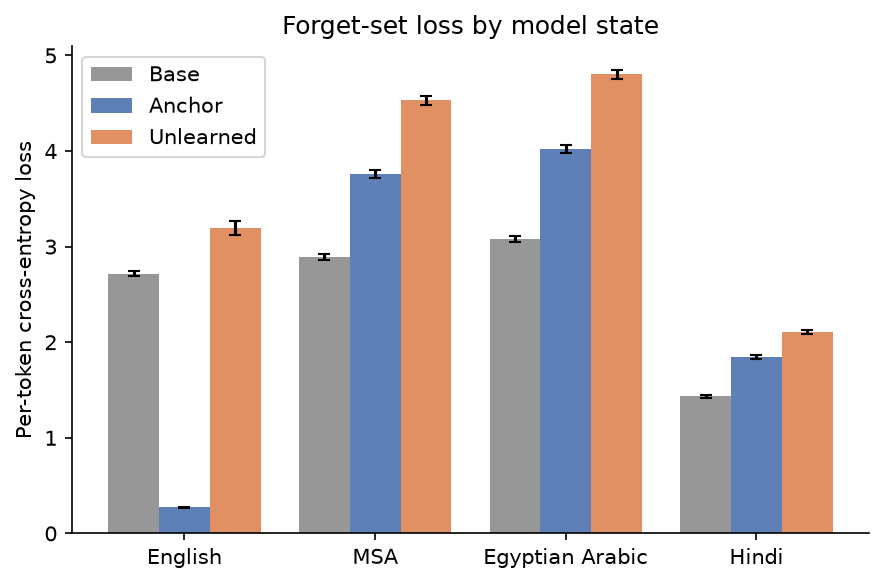
\includegraphics[width=\columnwidth]{fig_loss_by_state.png}
\caption{Forget-set loss by model state. The anchor falls far below the base
model in English — the facts were learned — and sits \emph{above} it in MSA,
Egyptian Arabic and Hindi, where English-only fine-tuning left the model
worse at those facts than before training. Unlearning then raises loss in
every variety, but only in English does it undo something the anchor had.
Error bars are $95\%$ bootstrap intervals over 400 facts.}
\label{fig:loss_by_state}
\end{figure}

\paragraph{The leakage signature is present.}
Read the way a standard audit reads it, our result is a textbook case of
cross-lingual leakage. Unlearning raises English forget-set loss by $+2.922$
nats, from $0.272$ to $3.194$ — the anchor's memorisation is undone, and the
model ends up above where the untuned base model was. In MSA the same
checkpoint moves only $+0.774$ nats, $26\%$ as far. Egyptian Arabic
($+0.778$) and Hindi ($+0.267$) look similar or weaker. A paper reporting
only these numbers would conclude that GradDiff erases in English while
leaving the facts recoverable in Arabic, and the effect sizes are large
enough that no amount of statistical care within that comparison would
overturn it.

\paragraph{The transfer control removes it.}
Step 1 of Table~\ref{tab:deltas}, plotted in Figure~\ref{fig:loss_by_state},
shows why that conclusion is not available.
Fine-tuning cut English forget-set loss by $-2.445$ nats, but in MSA it
\emph{raised} forget-set loss by $+0.870$, in Egyptian by $+0.941$ and in
Hindi by $+0.408$. The anchor is worse at predicting the Arabic and Hindi
forget facts than the model it was trained from. Whatever the $+0.774$-nat
MSA movement in Step 2 represents, it cannot be the removal of knowledge the
anchor did not have.

\paragraph{What movement remains is not fact-specific.}
The retain control locates the residue. In Step 1, MSA retain loss rose
$+0.886$ against forget's $+0.870$; Egyptian $+0.945$ against $+0.941$;
Hindi $+0.433$ against $+0.408$. English-only fine-tuning degrades these
languages globally — catastrophic forgetting of the target language, not
acquisition of the target facts — and the forget and retain sets are carried
along together. The nets are $-0.016 \pm 0.058$, $-0.003 \pm 0.060$ and
$-0.025 \pm 0.023$: no fact-specific transfer at any measurable level.

English is the instructive contrast, and it is why the Step 1 net must not be
read as an acquisition test. There too the two splits move together
($-2.445$ against $-2.500$, net $+0.055 \pm 0.075$), but for the opposite
reason: the anchor was trained on both, so what they share is learning rather
than drift. A net is informative only where the two splits were treated
differently. In Step 2 they were — forget under the ascent term, retain under
the descent term — so the net isolates fact-specific movement. In Step 1 they
were not, and acquisition has to be read off the raw forget-set change, which
is negative in English alone.

Read that way, Step 2 gives an MSA net of $+0.054 \pm 0.038$ and an Egyptian
net of $+0.046 \pm 0.039$; both exclude zero at $n=400$, but they are $2.5\%$
and $2.1\%$ of the English net of $+2.155 \pm 0.152$, and they sit on facts
for which the transfer control shows no acquisition. Hindi is
$-0.010 \pm 0.015$, indistinguishable from zero. The apparent MSA leakage
shrinks from $26\%$ of the English effect to $2.5\%$ once the never-learned
and drift components are taken out. Both figures are ratios of teacher-forced
loss movements, and loss movement is not a direct measure of how much of a
fact remains recoverable; what the comparison establishes is that the
movement attributable to the targeted facts in Arabic is a small fraction of
the English one, not that a specific fraction of knowledge survives.

\paragraph{No transfer at the level of individual facts either.}
The aggregate could in principle hide transfer on a subset of facts. It does
not. Correlating each fact's English unlearning delta with its delta in
another variety gives $r = +0.029$ for MSA, $+0.005$ for Egyptian and
$-0.038$ for Hindi. Facts that were forgotten hardest in English were not
forgotten harder anywhere else.

\begin{table}[t]
\centering
\small
\begin{tabular}{lrr}
\toprule
Variety & Never-trained $\Delta$ & Forget $-$ never-trained \\
\midrule
EN  & $+1.934$ & $-4.378 \pm 0.400$ \\
MSA & $+2.012$ & $-1.143 \pm 0.228$ \\
EGY & $+2.151$ & $-1.210 \pm 0.220$ \\
HI  & $+0.836$ & $-0.429 \pm 0.160$ \\
\bottomrule
\end{tabular}
\caption{Base $\rightarrow$ anchor movement on the 217 TOFU
\texttt{real\_authors} and \texttt{world\_facts} items, which no stage of our
pipeline trains on, and what subtracting it from the forget-set change would
imply. We report this baseline but do not apply it: see text.}
\label{tab:drift}
\end{table}

\paragraph{A never-trained drift baseline.}
The retain set is fine-tuned on, so in English it cannot measure drift. A
baseline the anchor never saw would separate the two, and TOFU supplies one:
the \texttt{real\_authors} and \texttt{world\_facts} splits, 217 items in
total, which no stage of our pipeline trains on. We translated them with the
same NLLB pipeline and probed them with the same adapters
(Table~\ref{tab:drift}). Fine-tuning moves them by $+1.934$ to $+2.151$ nats
in English, MSA and Egyptian Arabic, more than twice what it moves the
persona probes in any non-English variety, and subtracting that from the
forget-set change would imply that English-only fine-tuning taught the model
the facts in all three non-English varieties, Hindi included. We do not read it that way. The two sets differ in form:
answers in the never-trained splits average 3--11 tokens against 33--166 for
the persona answers, and fine-tuning on four thousand long biographical
sentences moves the model away from short factual answers in every language
at once. The baseline measures that shift, not the drift our probes undergo.

What the exercise does establish is when a retain control can be trusted. Our
anchor is fine-tuned in English alone, so outside English neither split was
ever trained on: the translated retain set is itself a never-trained baseline,
and unlike \texttt{world\_facts} it matches the forget probes in length and
register. That is why MSA forget ($+0.870$) and retain ($+0.886$) coincide so
closely. The contamination is confined to English, where both splits were
trained and where acquisition is therefore read off the raw change of
$-2.445$. The baseline this experiment reaches for would be persona facts
held out of fine-tuning altogether: never trained on, and matched to the
probes in length and register. That costs an anchor run, which is why we
report the mismatched baseline here and return to the matched one in
Section~\ref{sec:discussion}.

\paragraph{Robustness to the translation artefact.}
Restricting MSA to the 337 forget facts whose answers contain no Latin
script, which removes the untransliterated persona names and the
\emph{LGBTQ} acronym discussed in Section~\ref{sec:setup}, leaves the picture
unchanged: transfer $+0.885$ against a retain control of $+0.886$, and an
unlearning delta of $+0.764$ against $+0.774$ on the full set. The artefact we were most concerned about is not what produces the
null.

\paragraph{The null is not an underpowered one.}
At $n=400$ the confidence intervals on the non-English nets are narrow
enough to matter: $\pm 0.058$, $\pm 0.060$ and $\pm 0.023$ nats in Step 1,
against a Step 2 English net of $+2.155$. A transfer effect anywhere near
the magnitude of the English one would have been detected many times over.
What the data cannot exclude is an effect one to two orders of magnitude
smaller, which is the bound we claim rather than zero.

% ============================================================
\section{Discussion}
\label{sec:discussion}

\paragraph{Why the naive reading is so easy to believe.}
The failure mode is not a subtle statistical one. Every number an
anchor-versus-unlearned comparison produces in our setup points the same way:
a large English delta, a much smaller Arabic delta, a monotone ordering
across varieties, and hundreds of facts behind each mean. The comparison is
internally consistent and simply measures something other than what it is
taken to measure. It is also the comparison that comes for free — the base
model is the one artefact an unlearning pipeline has no other reason to
evaluate, since its role is normally discharged once, in the unlearning
language, to show the benchmark facts start out unknown.

\paragraph{Why transfer failed here.}
Two explanations are consistent with Step 1, and our data separate them only
partly. The first is capacity and typological distance: a 0.5B model with a
rank-16 adapter, trained on 4{,}000 English examples, may lack the shared
representation needed to make an English-learned fact predictable in
Arabic script. This is the direction \citet{farashah2026multilingual}
predict — they find syntactic similarity the strongest predictor of whether
unlearning transfers, and English and Arabic are remote in family, dominant
word order and morphological type. Consistent with a distance account, Hindi
moves least. The second is interference: fine-tuning hard on one language
degraded the others, and that degradation could be masking a small genuine
transfer effect. The retain control cannot distinguish these, because it
subtracts exactly the quantity that would be needed to see it, and the
never-trained baseline of Table~\ref{tab:drift} does not settle it either: it
moves too much, for reasons of form rather than language.

What we can say is that the confound in our setup is not resolved by
appealing to resourcing. MSA is the best-represented Arabic variety in both
the backbone's pretraining and NLLB's translation distribution, and it shows
no more transfer than Egyptian. Nor is the null an artefact of our
translations: it survives restriction to Latin-script-free answers, and it
appears identically on the retain set, which is drawn from the same
translation pipeline and is not targeted by any intervention.

\paragraph{Implications for evaluation.}
We do not claim cross-lingual leakage is not real; \citet{choi2024crosslingual}
and \citet{farashah2026multilingual} report it at larger scale and with
multilingual backbones, and nothing here contradicts them. We claim that the
evidence standard usually applied to it is too weak to distinguish it from
the case where transfer never occurred, and that in at least one reasonable
setup the weak standard returns a confident false positive. Three
requirements follow.

\begin{enumerate}
  \item Probe the base model in every language the audit reports, not once
overall.
  \item Probe a retain set alongside every forget set, so that fact-specific
movement can be separated from drift.
  \item Report $\Delta_v^{\text{tr}}$ as a precondition of the leakage claim,
measured on the forget set itself rather than net of the retain set, since
fine-tuning acts on both: where it does not show acquisition in variety $v$,
no statement about forgetting in $v$ is licensed.
\end{enumerate}

\noindent The cost is inference only, on adapters the pipeline already
produces.

\paragraph{What it would take to test leakage properly.}
The experiment our original question needs is an anchor that demonstrably
knows the facts in every probed variety — multilingual fine-tuning, with
unlearning still applied in English alone. That makes $\Delta_v^{\text{tr}}$
negative by construction and the leakage question well posed. It also costs
a second anchor: ours took 23.3 GPU-hours for the English one. Holding a
slice of the persona facts out of that run would, at no extra cost, also
supply the never-trained and format-matched drift baseline that
Table~\ref{tab:drift} approximates poorly. We regard this pair, rather than a
larger model, as the first thing to change.

A second axis worth varying is typological distance. Our three targets are
all remote from English, and a closer language — German, say — would test
whether the size of the transfer null tracks distance in the way
\citet{farashah2026multilingual} predict, or whether monolingual fine-tuning
at this scale simply fails to cross any language boundary.

% ============================================================
\section{Conclusion}
\label{sec:conclusion}

We set out to measure whether GradDiff unlearning of English TOFU facts
leaves those facts recoverable in Arabic, and obtained the expected answer:
an English forget-set loss increase of $+2.922$ nats against $+0.774$ in MSA,
$26\%$ as large. Adding a base-model measurement per variety showed the
comparison to be unsound. English-only fine-tuning raised forget-set loss in
MSA, Egyptian Arabic and Hindi rather than lowering it, and raised retain-set
loss by a statistically indistinguishable amount, leaving no measurable
fact-specific knowledge for unlearning to act on. Net of both controls the
MSA effect is $+0.054$ nats, $2.5\%$ of English, on facts the model cannot be
shown to have known in Arabic.

The methodological point generalises beyond our backbone. A cross-lingual
unlearning result is a claim about a difference between two languages, and it
needs a control establishing that the knowledge existed in both. We report
the full base\,$\times$\,anchor\,$\times$\,unlearned grid, crossed with
forget and retain probes, as the minimum sufficient design, and release the
harness that produces it by adapter hot-swapping on a single frozen base.

% ============================================================
% Unnumbered so it does not consume a section number.
\section*{Code and Data Availability}

The training, unlearning and audit code, the QLoRA adapter weights for the
anchor and unlearned checkpoints, and the machine-translated Arabic
evaluation sets are available at
\url{https://github.com/Waseem177/forgotten-in-msa}. The underlying TOFU
corpus is distributed by \citet{maini2024tofu} under the MIT licence, which
permits the redistribution of our translated derivative.

% ============================================================
% Unnumbered, placed after the Conclusion and before the references, where
% it does not count against the page limit.
\section*{Limitations}

The scope of our negative transfer result is bounded by a single backbone.
We selected \textsc{Qwen2.5-0.5B-Instruct} after establishing that
\textsc{Aya-Expanse-8B} could not be trained on our hardware: 4-bit
quantisation leaves the 256k-token embedding matrix in \texttt{bf16},
consuming roughly 2.1\,GB before any transformer weight loads. A 0.5B model
with modest Arabic capacity is a case where cross-lingual acquisition should
be hard, so ``fine-tuning implanted nothing in Arabic'' may not hold for a
larger or deliberately multilingual backbone. Our methodological claim does
not depend on this: the weaker the transfer, the more a leakage audit needs
the control that detects it. But readers should not take the null itself as a
general fact about LLMs.

The sharper form of that objection is that the variable which matters is not
parameter count but how much of each language the backbone saw in
pretraining, which for most open-weight models is undocumented. Recent fully
open releases that publish their training corpora alongside their weights
would allow the transfer control to be read against a known share of Arabic
rather than an assumed one, and we regard that as the more informative
replication.

Relatedly, our transfer control is a null result, and a null cannot be
distinguished from insufficient sensitivity by the measurement that produced
it. We report confidence intervals narrow relative to the English effect
(non-English nets within $\pm 0.06$ nats against an English unlearning
effect of $+2.155$), which bounds how large a
transfer effect could be hiding, but a fact-specific signal well below that
floor would be invisible to us.

We evaluate a single unlearning method. Gradient-difference unlearning has an
unbounded ascent term, and our runs pass through a narrow usable region before
diverging: at a learning rate of $1{\times}10^{-5}$ the forget loss moves from
$0.30$ to $1.02$ to $4.59$ and then to $57.8$ over four epochs. We select a
checkpoint from within that region, so our results characterise a
deliberately-chosen operating point rather than the method's behaviour
throughout training. Bounded objectives such as NPO \citep{zhang2024npo} may
leak differently.

Our non-English probes are machine-translated with NLLB-200
\citep{nllbteam2022nllb} rather than produced by native speakers. A translation
artefact could depress apparent recall in a target language and be
indistinguishable from genuine forgetting. We mitigate this with a
native-speaker check of the Modern Standard Arabic probes, but the Egyptian
Arabic and Hindi probes carry this risk unquantified, and NLLB's dialectal
Arabic is weaker than its MSA.

We measure forgetting by teacher-forced loss on the reference answer, not by
what the model generates. This cuts in both directions here. A model may
score a high loss on the gold answer while still emitting the memorised fact
under sampling; equally, knowledge may be present in a form that raises no
signal on one particular translated string. Our transfer control inherits
that weakness, so ``no measurable acquisition under a loss probe'' is a
weaker statement than ``no acquisition''. Generation-based metrics and
adversarial extraction, in the manner of \citet{doshi2024unlearn}, would
tighten the control as much as they tighten the audit.

Finally, TOFU consists of synthetic facts about fictional authors, which is
what makes clean forget/retain control possible, and it is also the reason
our setup is the hardest possible case for transfer: the model meets these
facts only during English fine-tuning, and only in English. Real personal
data is redundantly attested across a pretraining corpus in many languages at
once, so knowledge genuinely does exist in multiple languages there and the
leakage question is well posed in a way it is not here. That is a limitation
on our null, not on our argument for the control — a real-data audit that
omits the transfer control still cannot show which of its languages held the
fact.

% ============================================================
\section*{Acknowledgments}

We thank the MRL 2026 organisers for their help and flexibility during the
submission process. We also thank the anonymous reviewers: the never-trained
drift baseline in Table~\ref{tab:drift} was run at their suggestion, and the
discussion of when a retain control can be trusted is sharper for it.

% ============================================================
\bibliography{refs}

\end{document}
